\documentclass[11pt]{article}

\usepackage{appendix}
\usepackage{array}
\usepackage{parskip}
\usepackage{graphicx}
\usepackage{amsmath}
\usepackage{listings}

\usepackage[T1]{fontenc}
\usepackage{lmodern}
\usepackage[autostyle, english = american]{csquotes}
\MakeOuterQuote{"}

\newcolumntype{L}[1]{>{\arraybackslash}m{#1}}

\usepackage{pythonhighlight}

% Margins
\topmargin=-0.45in
\evensidemargin=0in
\oddsidemargin=0in
\textwidth=6.5in
\textheight=9.0in
\headsep=0.25in

\title{605.744: Information Retrieval \\ Programming Assignment \#3: Inverted Files}
\author{Sabbir Ahmed}
\date{\today}

\begin{document}
\maketitle	
\tableofcontents
\clearpage
\newpage

\section{Introduction}
This paper describes the enhancements and features added to the Information Retrieval program started in Assignment 1 and upgraded in Assignment 2. Modifications include improvement in performance and adding support for batch processing and ranking queries.

\section{Technical Background}
All of the source code is in Python 3.10. The program is split into several modules and follows an object oriented structure. The following is the directory structure of the source code:

% .
% ├── bin/
% ├── ir/
% │   ├── const.py
% │   ├── files.py
% │   ├── __init__.py
% │   ├── invertedfile.py
% │   ├── lexer.py
% │   ├── normalize.py
% │   ├── packer.py
% │   ├── retriever.py
% │   └── types.py
% ├── run.py
% ├── stats/
% └── tmp/

\begin{figure}[!ht]
    \centering
    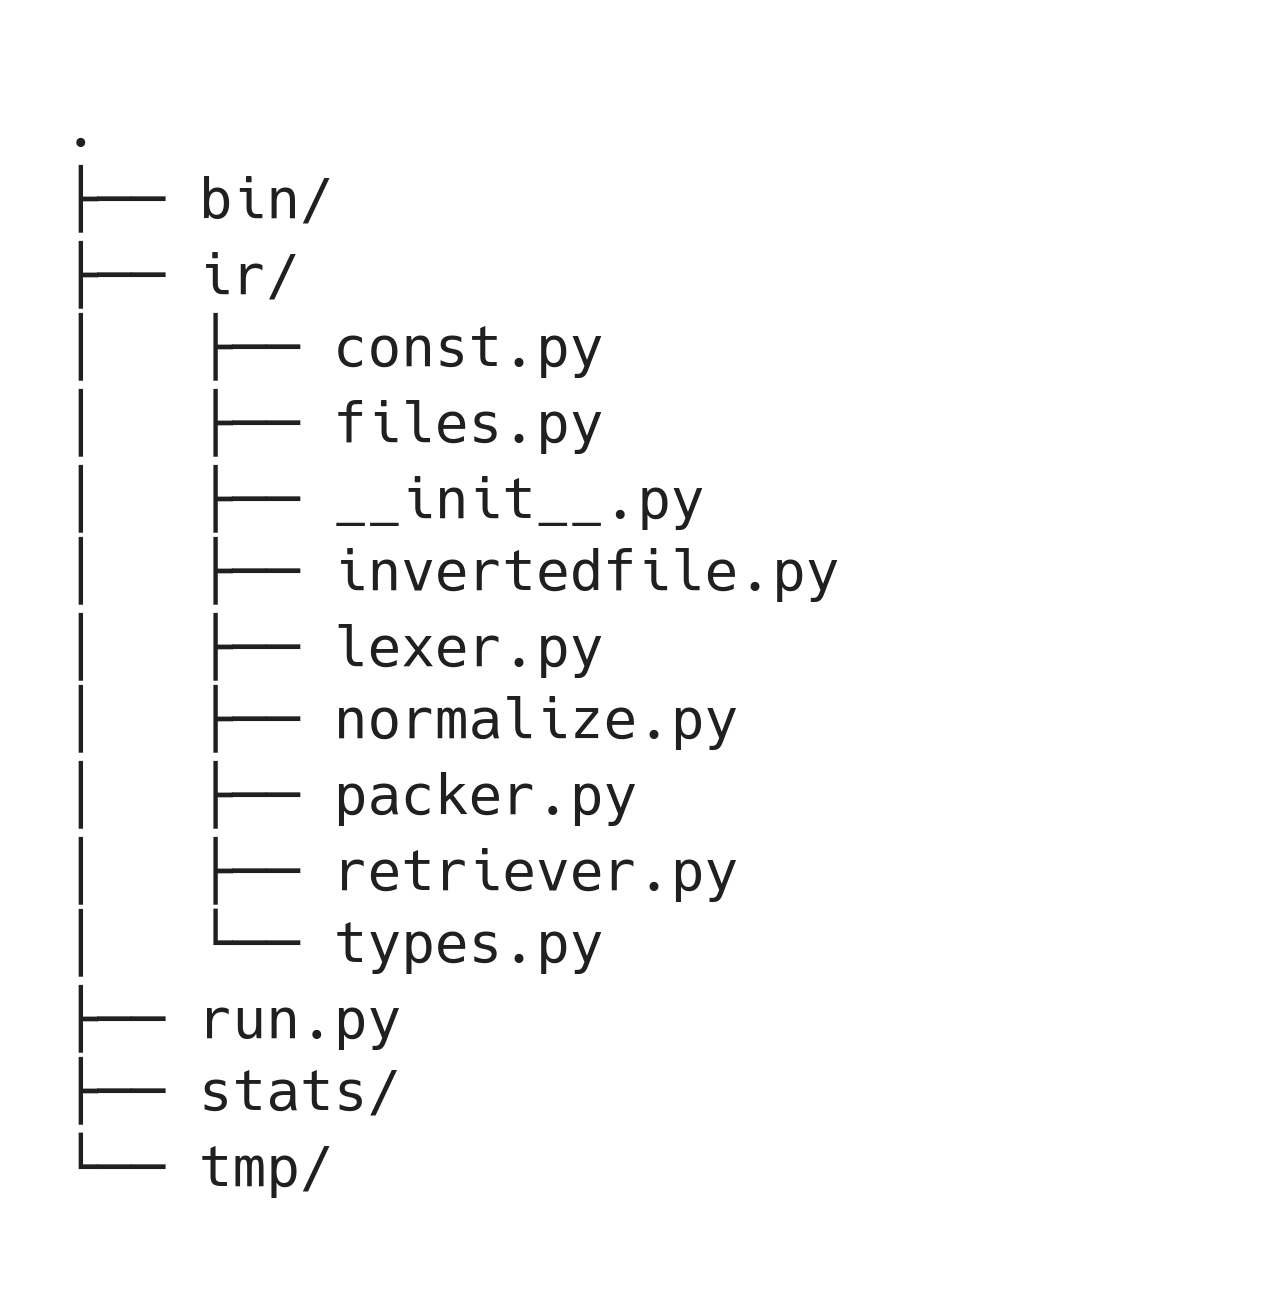
\includegraphics[scale=0.2]{statics/dirtree.png}
    \caption{Directory Hierarchy of Assignment 3}
\end{figure}

The source code for all of the files are attached in Appendix \ref{appendix:src}.

The total number of non-empty lines of code for the program totals to under 750.

\begin{figure}[!ht]
    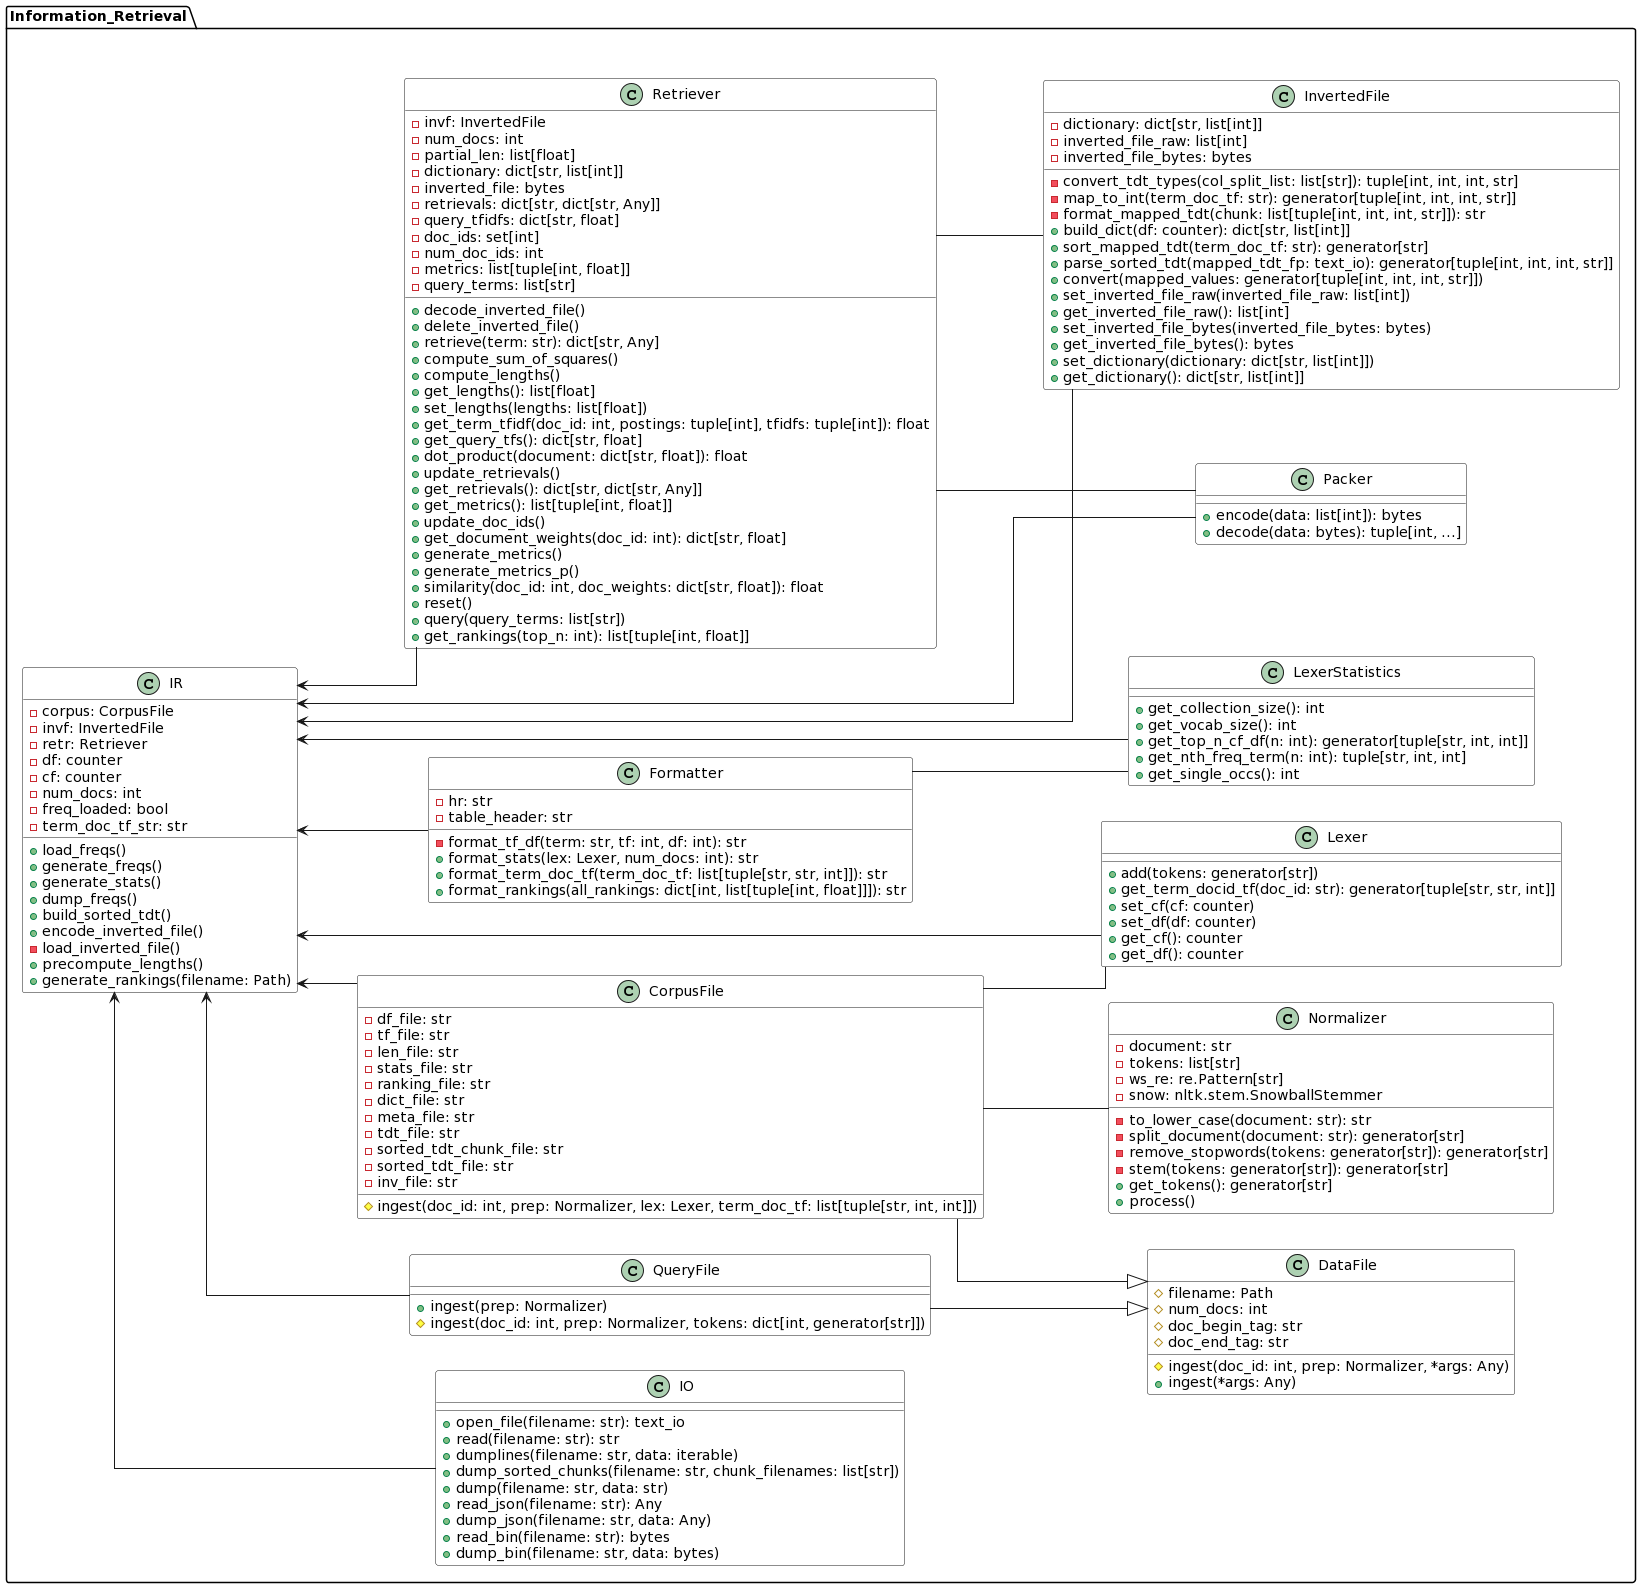
\includegraphics[scale=0.31]{statics/uml.png}
    \centering
    \caption{UML of Information Retrieval}
\end{figure}

\subsection{Existing Classes}

\subsubsection{Driver} \label{sec:driver}
The driver script for the program is \texttt{run.py}. The script uses command line options to process corpus files to perform the following operations:

\begin{enumerate}
    \item generate document and relative term frequencies
    \item generate statistics on corpus frequencies
    \item save frequencies to file
    \item extract term-docID-term frequency records and save to temporary files
    \item generate, encode and save inverted file
    \item compute document weights and save for repeated use
    \item process query files and generate rankings
\end{enumerate}

\subsubsection{\texttt{lexer} Classes}
The \texttt{Lexer} class had its methods on generating statistics separated into the \texttt{LexerStatistics} class.

\subsubsection{\texttt{files} Classes}
The \texttt{DataFile} class was renamed to \texttt{CorpusFile} and the \texttt{QueryFile} class was added to ingest query files. Both of these classes have been derived from the \texttt{DataFile} class.

The \texttt{Formatter} class has a new method to format rankings.

The \texttt{IO} class has a new method for writing chunks of data to files to be merged again. This method is only used for dumping chunks of sorted term-docID-term frequency records.

\subsubsection{\texttt{invertedfile.InvertedFile}}
The \texttt{InvertedFile} class received the following modifications:
\begin{itemize}
    \item the dictionary now only contains the term index, offset, length, and document frequency for each terms.
    \item the term-docID-term frequency records were sorted and saved to files in chunks. The chunk files are later merged to a single sorted file. This approach allows for the program to process  large corpuses without stressing the memory.
\end{itemize}

\subsection{New Classes}

\subsubsection{\texttt{retriever.Retriever}}
The\texttt{Retriever} class was added to compute document weights and rank queries.

The class precomputes document lengths to save to a file for repeated use. The document lengths are computed by reading the pre-generated inverted file and walking through each of the terms in the dictionary. The partial lengths of the documents are computed by adding the square of the TF-IDF of each of the term. The TF-IDF of a term is the product of its term frequency saved in the postings list of the inverted file and the logarithm of the inverse of its postings length. Once the entire inverted file is processed, the square root of each of the document partial lengths are computed and stored to file as the document vector lengths.

Once the document lengths have been computed, the class can process queries to compute similarities between its term weights against all of the documents in the corpus to generate rankings. The rankings are based on the cosine similarities between the query and the documents. The similarities are determined by evaluating the dot product of the query with each of the "relevant" documents and dividing the value with the product of their lengths. A document is considered "relevant" if it contains at least one of the query terms.

Generating this ranking is computationally expensive, even with the precomputed document lengths. The rankings of the query prompts were generated on a Debian-based Linux virtual machine with 2 cores, and generating the top 100 rankings for 50 queries per file may take hours to execute serially. Therefore, the class has been optimized to compute weights in parallel if the number of relevant documents exceed a threshold. The threshold value is assigned arbitrarily; 75,000 documents for \textit{cord19.topics.keyword.txt} and 90,000 documents for \textit{cord19.topics.question.txt}.

\subsection{Output Files}
With the addition of several processes that rely on saving progress by writing no disk, the program makes use of numerous temporary files. The following table provides descriptions of each of the files:

\begin{table}[!ht]
    \caption{Description of the files used by the program}
    \begin{center}
        
        \begin{tabular}{| L{3.5cm} | L{12cm} |}
        \hline
        \textbf{File name} & \textbf{Description}
        \\ \hline
        corpus\_df.txt & Document frequencies of each normalized terms in the dictionary in the format: \newline \texttt{\{"bird": 8, "dog": 4, ...\}}
        \\ \hline
        corpus\_cf.json & Relative term frequencies of each normalized terms in the dictionary in the format: \newline \texttt{\{"bird": 21, "dog": 10, ...\}}
        \\ \hline
        corpus\_summary.txt & Summary statistics of the corpus as described in Assignment 1
        \\ \hline
        corpus\_len.json & Vector lengths of each of the documents in the corpus in the format: \newline \texttt{{[0.0, 3.0, 3.7416573867739413, ...]}}
        \\ \hline
        corpus\_rank.txt & Rankings generated from a query file sorted and formatted as described in the prompt
        \\ \hline
        corpus\_dict.json & Dictionary of the corpus containing each of the normalized terms mapping to their term index, inverted file offset, inverted file postings width, and their document frequency in the format: \newline \texttt{\{"aardvark": [0, 0, 8, 4], "bird": [1, 8, 16, 8], ...\}}
        \\ \hline
        corpus\_ndocs.txt & Number of documents in the corpus; this value is saved on disk to avoid having to reading large corpuses multiple times
        \\ \hline
        corpus\_tdt.txt & The term-docID-term frequency records saved to file after the entire corpus is processed in the format: \newline \texttt{bird 1 1 \newline
        dog 1 3 \newline
        aardvark 2 1 \newline
        ...}
        \\ \hline
        corpus\_chunk\_$i$.txt ($i=0$ to $N$) & The sorted chunks of \texttt{corpus\_tdt.txt}; each of these  $N$ files are limited to \texttt{const.CHUNK\_SIZE} lines in the format: \newline \texttt{0 2 1 aardvark \newline
        0 3 5 aardvark \newline
        0 4 2 aardvark \newline
        0 8 1 aardvark \newline
        1 1 1 bird \newline
        1 2 2 bird \newline
        ...}
        \\ \hline
        corpus\_sort.txt & The final sorted \texttt{corpus\_tdt.txt} file after merging all of its sorted chunks
        \\ \hline
        corpus\_if.bin & The inverted index file of the corpus
        \\ \hline
        \end{tabular}

    \end{center}

\end{table}

\subsection{Constants}
The following constants are used in the program:

\begin{table}[!ht]
    \caption{Description of the constants used by the program. All of the values are located in \texttt{const.py}}
    \begin{center}

        \begin{tabular}{| L{4cm} | L{1.5cm} | L{9cm} |}
        \hline
        \textbf{File name} & \textbf{Value} & \textbf{Description}
        \\ \hline
        DOC\_PROC & 10,000 & Used by the \texttt{Formatter} class to report progress on corpus normalization
        \\ \hline
        CHUNK\_SIZE & 1,000,000 & Maximum number of lines of term-docID-term frequency records to sort in memory before writing to disk
        \\ \hline
        BYTE\_FMT\_CHAR & "I" & The format of bytes in the inverted index file
        \\ \hline
        BYTE\_FMT\_SIZE & 4 & The size of an integer in the binary inverted index file
        \\ \hline
        QUERY\_DOC\_ID & 0 & Used by the \texttt{Retriever} class; this index is reserved in the final document vector length list for the query weights
        \\ \hline
        PARALLEL\_THRESH & 75,000  90,000 & arbitrary thresholds to determine when to generate rankings in parallel
        \\ \hline
        IDX.TID & 0 & Used by the corpus dictionary and inverted index file; index of the term in the dictionary
        \\ \hline
        DICT.OF & 1 & Used by the corpus dictionary; index of the file offset of the term in the inverted file
        \\ \hline
        DICT.WID & 2 & Used by the corpus dictionary; index of the length of the postings list of the term in the inverted file
        \\ \hline
        DICT.DF & 3 & Used by the corpus dictionary; index of the document frequency of the term
        \\ \hline
        INVF.DID & 1 & Used by the inverted index file; index of the document ID
        \\ \hline
        INVF.TF & 2 & Used by the inverted index file; index of the frequency of the term in the document
        \\ \hline
        INVF.STR & 3 & Used by the inverted index file; index of the term string used to match values in the dictionary and compute postings lengths
        \\ \hline
        \end{tabular}

    \end{center}

\end{table}
\newpage

\section{Statistics}
The following table details the storage used by the dictionary and inverted index files of \texttt{cord19.txt}; the combined space they occupied on disk are significantly lower than the corpus document.

\begin{table}[!ht]
    \caption{Sizes of files computed through the \texttt{stat} command on a Debian-based Linux}
    \begin{center}

        \begin{tabular}{| l | r | l |}
        \hline
        \textbf{File} & \textbf{Size (in bytes)} & \textbf{Description} \\
        \hline
        cord19.txt & 359,302,564 & Input corpus file
        \\ \hline
        cord19\_dict.json & 8,830,004 & Generated dictionary JSON file
        \\ \hline
        cord19\_if.bin & 145,476,192 & Binary inverted index file
        \\ \hline
        cord19\_len.json & 3,717,192 & Precomputed document lengths
        \\ \hline
        \end{tabular}

    \end{center}

\end{table}

The following is the processed query terms and their weights of the first query of \textit{cord19.topics.keyword.txt}, "coronavirus origin":

% {"coronavirus": 1.9400969473898837, "origin": 4.1451228967712135}

\begin{table}[!ht]
    \caption{Term weights of the query "coronavirus origin"}
    \begin{center}

        \begin{tabular}{| c | c |}
        \hline
        \textbf{Normalized term} & \textbf{Weight}
        \\ \hline
        "coronavirus" & 1.9400969473898837
        \\ \hline
        "origin" & 4.1451228967712135
        \\ \hline
        \end{tabular}

    \end{center}

\end{table}

The rankings of \texttt{cord19.topics.keyword.txt} and \texttt{cord19.topics.question.txt} were generated in independent executions.

\subsection{\texttt{cord19.topics.keyword.txt}}
The program took 998.231 seconds (approximately 16 minutes 38 seconds) in total to generate the rankings for the \texttt{cord19.topics.keyword.txt} queries. The following tables provide summary statistics of the queries and their executions:

% {"ndocs": {"max": 121750, "mean": 66226.86, "median": 61488.0, "min": 49993},
%  "nqueries": {"max": 4, "mean": 2.88, "median": 3.0, "min": 2},
%  "queries": [("coronavirus", 40),
%              ("covid", 7),
%              ("impact", 4),
%              ("test", 3),
%              ("respons", 2),
%              ("immun", 2),
%              ("mask", 2),
%              ("vaccin", 2),
%              ("sar", 2),
%              ("cov", 2)],
%  "time": 1118.231}

\begin{table}[!ht]
    \caption{Statistics of query rankings of \texttt{cord19.topics.keyword.txt}}
    \begin{center}

        \begin{tabular}{| c | c | c |}
        \hline
        \textbf{Metric} & \textbf{Relevant Documents Retrieved} & \textbf{Terms in Query}
        \\ \hline
        Minimum & 49,993 & 2
        \\ \hline
        Maximum & 121,750 & 4
        \\ \hline
        Mean & 66,226.86 & 2.88
        \\ \hline
        Median & 61,488.0 & 3.00
        \\ \hline
        \end{tabular}

    \end{center}

\end{table}

The following is the top 10 terms occurring in the  \texttt{cord19.topics.keyword.txt} query terms:

\begin{table}[!ht]
    \caption{Top 10 terms occurring in the \texttt{cord19.topics.keyword.txt} query terms}
    \begin{center}

        \begin{tabular}{| c | c |}
        \hline
        \textbf{Term} & \textbf{Number of Occurrences}
        \\ \hline
        "coronavirus" & 40
        \\ \hline
        "covid" & 7
        \\ \hline
        "impact" & 4
        \\ \hline
        "test" & 3
        \\ \hline
        "respons" & 2
        \\ \hline
        "immun" & 2
        \\ \hline
        "mask" & 2
        \\ \hline
        "vaccin" & 2
        \\ \hline
        "sar" & 2
        \\ \hline
        "cov" & 2
        \\ \hline
        \end{tabular}

    \end{center}

\end{table}

\subsection{\texttt{cord19.topics.question.txt}}
The program took 2176.277 seconds (approximately 36 minutes 16 seconds) in total to generate the rankings for the \texttt{cord19.topics.question.txt} queries. The following tables provide summary statistics of the queries and their executions:

% {'ndocs': {'max': 155723, 'mean': 101510.12, 'median': 105624.5, 'min': 39811},
%  'nqueries': {'max': 16, 'mean': 5.88, 'median': 5.0, 'min': 2},
%  'queries': [('covid', 31),
%              ('sar', 9),
%              ('cov', 9),
%              ('coronavirus', 8),
%              ('infect', 6),
%              ('impact', 6),
%              ('test', 4),
%              ('relat', 4),
%              ('prevent', 4),
%              ('complic', 4)],
%  'time': 2176.277}

\begin{table}[!ht]
    \caption{Statistics of query rankings of \texttt{cord19.topics.question.txt}}
    \begin{center}

        \begin{tabular}{| c | c | c |}
        \hline
        \textbf{Metric} & \textbf{Relevant Documents Retrieved} & \textbf{Terms in Query}
        \\ \hline
        Minimum & 39,811 & 2
        \\ \hline
        Maximum & 155,723 & 16
        \\ \hline
        Mean & 101,510.12 & 5.88
        \\ \hline
        Median & 105,624.5 & 5.00
        \\ \hline
        \end{tabular}

    \end{center}

\end{table}

The following is the top 10 terms occurring in the  \texttt{cord19.topics.question.txt} query terms:

\begin{table}[!ht]
    \caption{Top 10 terms occurring in the \texttt{cord19.topics.question.txt} query terms}
    \begin{center}

        \begin{tabular}{| c | c |}
        \hline
        \textbf{Term} & \textbf{Number of Occurrences}
        \\ \hline
        "covid" & 31
        \\ \hline
        "sar" & 9
        \\ \hline
        "cov" & 9
        \\ \hline
        "coronavirus" & 8
        \\ \hline
        "infect" & 6
        \\ \hline
        "impact" & 6
        \\ \hline
        "test" & 4
        \\ \hline
        "relat" & 4
        \\ \hline
        "prevent" & 4
        \\ \hline
        "complic" & 4
        \\ \hline
        \end{tabular}

    \end{center}

\end{table}

\section{Observations}
The rankings for \texttt{cord19.topics.keyword.txt} and \texttt{cord19.topics.question.txt} were saved on disk as \texttt{sahmed80-a.txt} and \texttt{sahmed80-b.txt} respectively. All of the queries across both of the files generated at least 100 rankings. Some interesting observations can be made on the similarity scores of the 2 files. The following table describes the frequencies of very low and very high similarity scores found in the rankings:

\begin{table}[!ht]
    \caption{Frequencies of very low and very high similarity scores generated in the top 100 rankings of the query files}
    \begin{center}

        \begin{tabular}{| c | c | c |}
        \hline
        \textbf{File} & \textbf{score $\leq 0.1$} & \textbf{score $\geq 0.9$}
        \\ \hline
        \texttt{sahmed80-a.txt} & 42 & 39
        \\ \hline
        \texttt{sahmed80-b.txt} & 180 & 5
        \\ \hline
        \end{tabular}

    \end{center}

\end{table}

It appears that the number of terms in the queries is inversely proportional to the similarity scores for their rankings.

\newpage
\clearpage

\appendix
\addcontentsline{toc}{part}{Appendix}%

\section{Source Code} \label{appendix:src}

\inputpython{../ir/files.py}{ir/files.py}
\inputpython{../ir/invertedfile.py}{ir/invertedfile.py}
\inputpython{../ir/lexer.py}{ir/lexer.py}
\inputpython{../ir/normalize.py}{ir/normalize.py}
\inputpython{../ir/packer.py}{ir/packer.py}
\inputpython{../ir/retriever.py}{ir/retriever.py}
\inputpython{../ir/types.py}{ir/types.py}

\inputpython{../run.py}{run.py}

\section{Outputs} \label{appendix:outputs}

\lstinputlisting[caption=Statistics of "cord19.txt",basicstyle=\small]{../outputs/stats/cord19_summary.txt}

\end{document}
